\section{Contribution}
\label{sec:contribution}

In the following, we will describe the details of how the business model of CCaaS exactly works.
We will first describe the contribution of CCaaS and the innovating company LinkedIn to the ecosystem,
i.e., what is the contribution of LinkedIn, what is the uniqueness of the contribution and why is 
LinkedIn suited to orchestrate the activities and resources for the CCaaS
\citep[p.~200-203]{schwafertsLectureStrategicBusiness2023}. This is part of the assessment of the
business model in the adjusted Business Model Canvas introduced in Section \ref{sec:business_model}.
We will then assess the novelty of the solution, before taking a closer look at the functionality, the
pricing and the system architecture of the offering.

\subsection{Value Chain and Contribution to the Ecosystem}

The contribution of CCaaS to the ecosystem is the creation of a new digital ecosystem for AI-based
career counseling. The uniqueness of CCaaS is mostly determined by access to data and access to
machine learning technology. Because LinkedIn is in a ``power play'' position in terms of breadth and
depth of data, it is uniquely positioned to offer such a service by leveraging on this data and AI
technology. Career counselors are typically not in a position to leverage on such data and technology. However,
they have the expertise to interpret the results of the AI models and to provide personalized services 
to the clients. As we have seen before, our persona of a career counselor is a highly educated person
that could be anxious about the impact of AI on the job market. The counselors are thus an important 
piece in the value chain to deliver the value to the customer. Therefore, LinkedIn's position is also 
limited and we can truly speak about a digital ecosystem (LinkedIn is not capable to deliver the 
counseling services on its own to the customer, as customer may not want fully automated services). 
Figure \ref*{fig:value_chain} shows the value chain in the digital ecosystem of AI-based career 
counseling.

\begin{figure}[h!]
    \centering
    \caption{Value chain in the digital ecosystem of AI-based career counseling.}
    \label{fig:value_chain}
    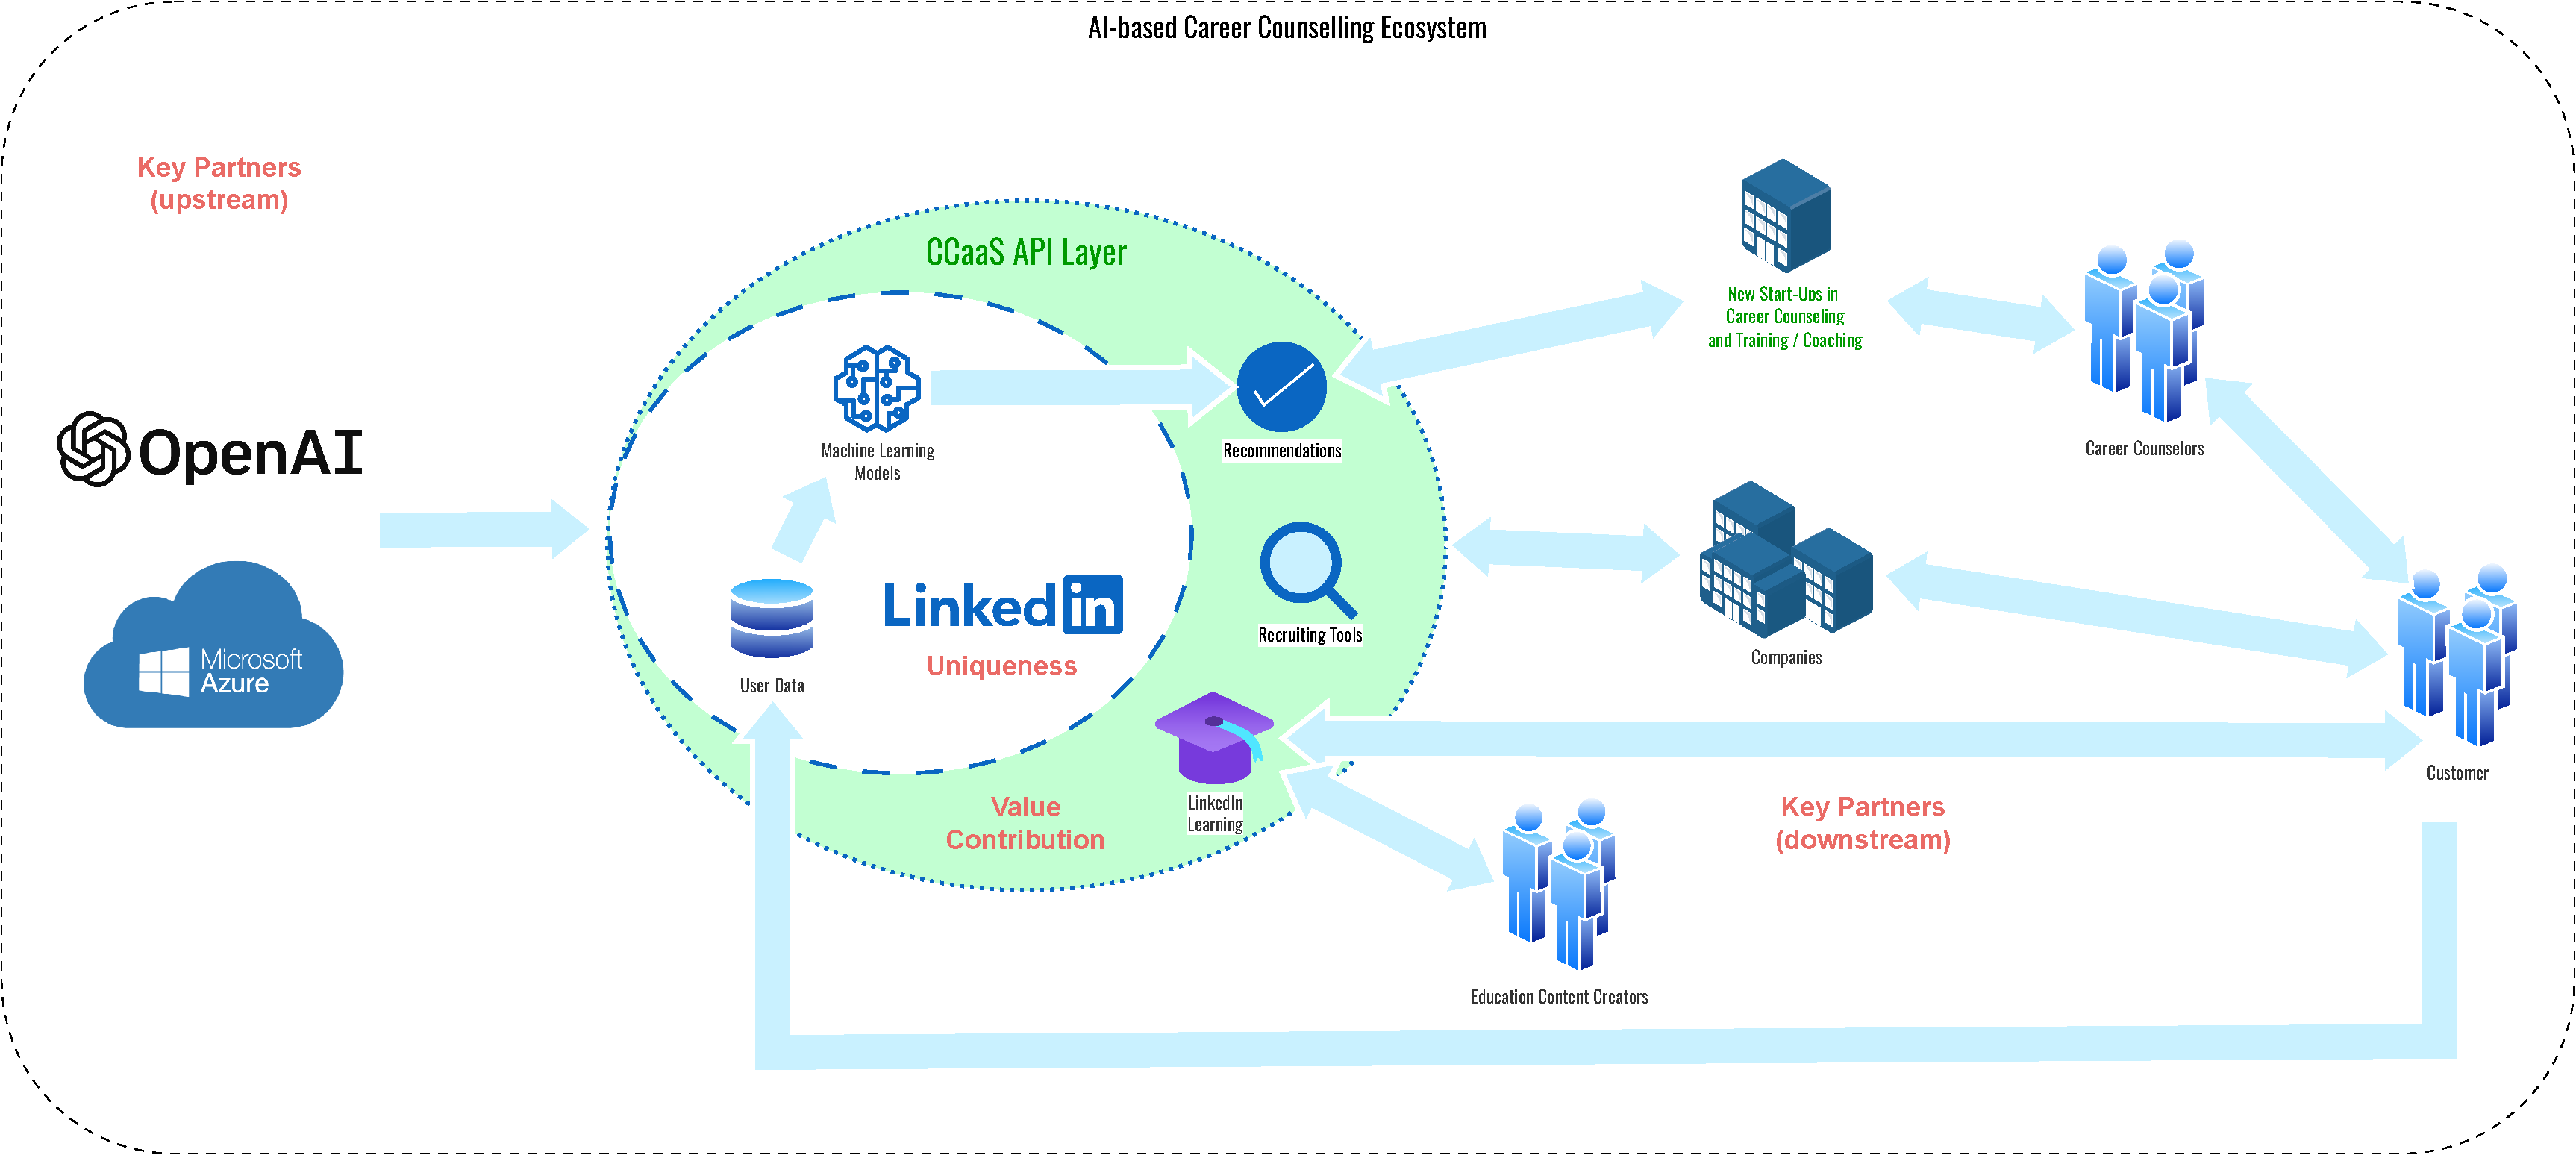
\includegraphics[width=\textwidth]{figures/value-chain.pdf}
\end{figure}

\subsection{Novelty}

The idea of offering career counseling as online services is not novel. Neither is the idea of
using AI models to assess a person's skills and interests, or to recommend suitable jobs and training
opportunities based on a user's profile. In fact, 44\% of jobs advertised on LinkedIn are already
filled using skills data as part of the recruitment process \citep{kaserAIpoweredCareerCounseling2023}.
This can typically be achieved by creating word embeddings of the job descriptions and the candidate's
profile (i.e., converting both to vector space), and using a similarity measure between the
vectors. Such vector similarity searches can even be implemented with off-the-shelf vector database
software, such as Weaviate \citep{dilockerWeaviate2023}. However, the idea of offering a platform that
provides career counseling as a service (CCaaS) is novel in several regards:

\begin{itemize}
    \item The CCaaS business model encourages co-creation of value based on data from LinkedIn and
        personalized services from career counselors.
    \item Offering CCaaS via an API layer enables integration with existing career counseling services.
    \item The CCaaS API layer enables counselors to build their own applications on top of the platform.
    \item Using the CCaaS API layer career counseling companies are encouraged to use a mix-and-match approach,
        where they can choose to use the AI models provided by CCaaS, use their own AI models for certain 
        use cases, or combine the CCaaS API services with services from other APIs (e.g., integrating 
        the training recommendation service with a training provider's API such as Coursera).
    \item The CCaaS business model leverages on the unique database of LinkedIn to create the best AI
        models for career counseling, while encouraging feedback data from the community of counselors
        and clients to further improve the AI models.
    \item Heavy investments in training the AI models is shared across all users of the platform
        via the API usage fees.
    \item The CCaaS API approach could fuel further innovation by enabling third-party developers to
        build their own applications on top of the platform, including building applications for 
        niche markets.
\end{itemize}

\subsection{Customer Journey Design}

Figure \ref{fig:blueprint_entrant} shows the service blueprint for the customer journey of a job
market entrant using career counseling via CCaaS. The service blueprint is a tool for service design
that describes the customer journey in terms of user actions and was introduced by \citet{shostackDesigningServicesThat1984}.
The service blueprint shows how the user actions connect to the frontstage, backstage, and internal
support services. User interactions are the actual actions undertaken by the customer to request or
consume the service, frontstage includes the visible touchpoints with the customer, while backstage
includes the processes that are not visible to the customer but utilized to render the service to the
customer. Finally, internal support services include the processes that are not visible to the customer
and not directly involved in the service delivery, but are required to support the service delivery.

The customer journey starts with the job market entrant (i.e., client) matching with a counselor
via the LinkedIn matchmaking web application. By choosing a counselor, the client automatically
grants access to its LinkedIn user profile data via the CCaaS API. The counselor can then access
the client's user profile data and start the actual counseling process. The counseling process
consists of an assessment of skills and values, retrieving job recommendations, and helping the
client choose the jobs to apply for using the profile data and leveraging on the CCaaS services
API endpoints. The writing assistance service---which is embedded in the existing job application
forms on LinkedIn---helps the client to write a better CV and application letters tailored to the
advertised positions and the client's profile. Finally, clients and counselors can leave feedback
on the recommendations and the counseling process via the LinkedIn matchmaking web application.
This feedback data flows back into the AI model training process.

To understand the full extent of the CCaaS offering, we also need to look at the customer journey
for a career transition. This customer journey aims at optimizing the career path of a client and
starts with a renewed assessment (leaving the counselor matchmaking aside). Based on the assessment
an optimal career path can be identified. However, the client may lack some skills or certifications
to advance in this new career path. This calls for an additional service of training recommendations
so that such skills gaps can be filled. Once the client has completed its additional training, the
counselor and AI models can help the client to find suitable jobs in the new career path. Finally,
counselors and clients can again leave feedback data for LinkedIn on the services and recommendations.
Figure \ref{fig:blueprint_transition} shows the service blueprint for the customer journey of a 
career transition.

\subsection{Pricing}

The pricing model for CCaaS is based on a pay-per-use model, where the API usage is metered and
charged to the counseling companies on a monthly basis. Each call on the API layer is logged via
a message broker and a logging microservice (see Subsection \ref{subsec:system_architecture}).
A separate microservice is connected with the billing and charging system of LinkedIn, and issues monthly
bills to the counseling companies based on the effective API usage in that month. API requests
can have different prices per request, depending on which API endpoint is used (i.e., what microservice
is called). The pricing model is based on the value that the API endpoint provides to the counseling
companies and the complexity of the AI models that are underlying the service. Table \ref{tab:pricing}
shows the proposed pricing model.

\begin{table}[h!]
    \centering
    \caption{API usage pricing by CCaaS API endpoint.}
    \label{tab:pricing}

    \tiny
    \renewcommand{\arraystretch}{1.1}
    \small\setlength\tabcolsep{8pt}

    \begin{tabularx}{0.8\linewidth}{X X X}
        \toprule
        \textbf{API Endpoint} &
        \textbf{Price} &
            \textbf{Proportion of Requests} \\
        \toprule

        Retrieve user data &
            1.00 USD p. user &
            20\% \\ 
        \midrule
        
        Skills and values assessment &
            3.00 USD p. assessment &
            15\% \\ 
        \midrule

        Job recommendation &
            0.25 USD p. job &
            50\% \\ 
        \midrule

        Training recommendation &
            0.50 USD p. training &
            10\% \\
        \midrule

        Career path recommendation &
            5.00 USD p. career path &
            5\% \\ 
        \bottomrule
    \end{tabularx}
\end{table}

\begin{landscape}
    \begin{figure}[h!]
        \centering
        \caption{Service blueprint for the job market entry customer journey. Blue: LinkedIn, orange: counselors (own illustration).}
        \label{fig:blueprint_entrant}
        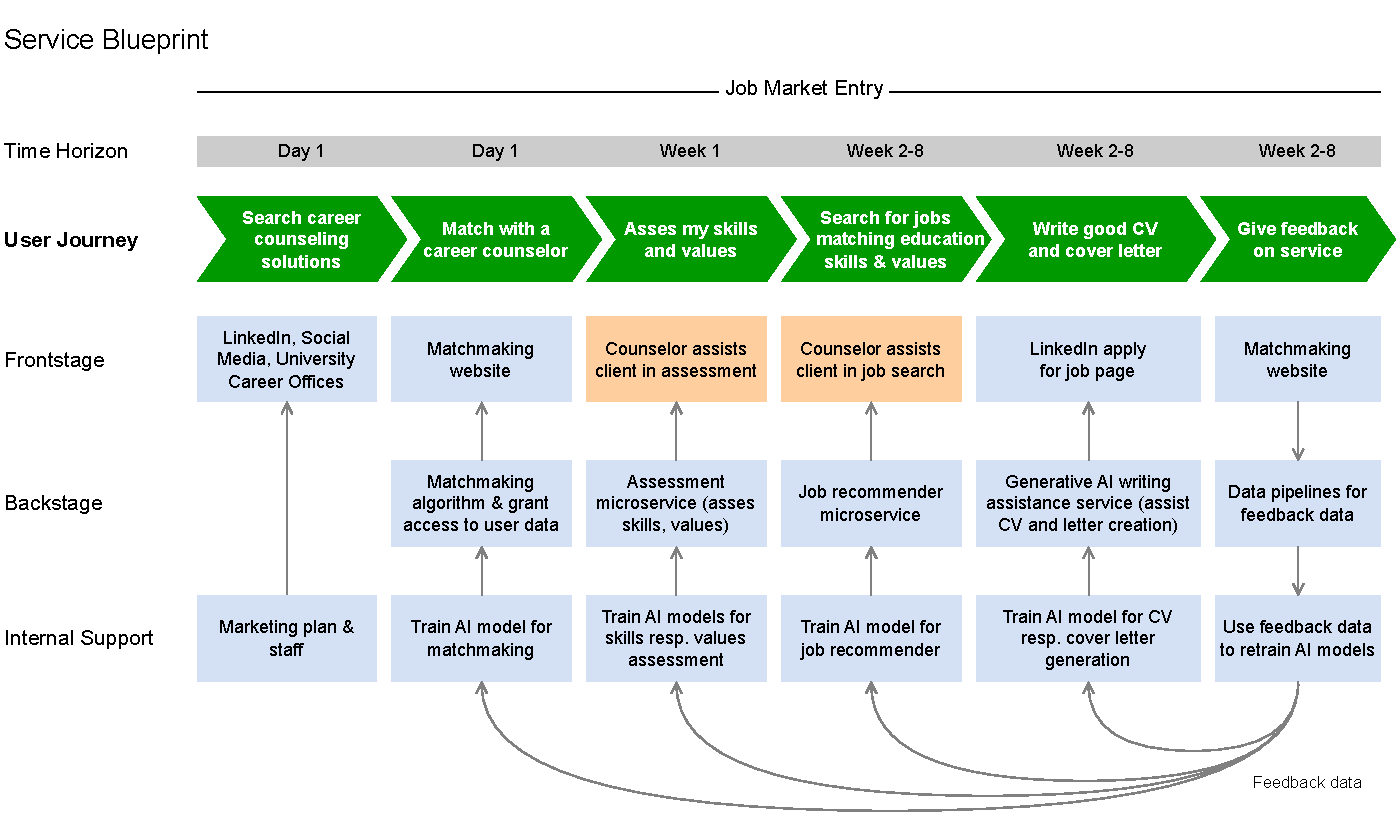
\includegraphics[width=\textwidth]{blueprint_entrant.pdf}
    \end{figure}
    
    \newpage

    \begin{figure}[h!]
        \centering
        \caption{Service blueprint for the career transition customer journey. Blue: LinkedIn, orange: counselors (own illustration).}
        \label{fig:blueprint_transition}
        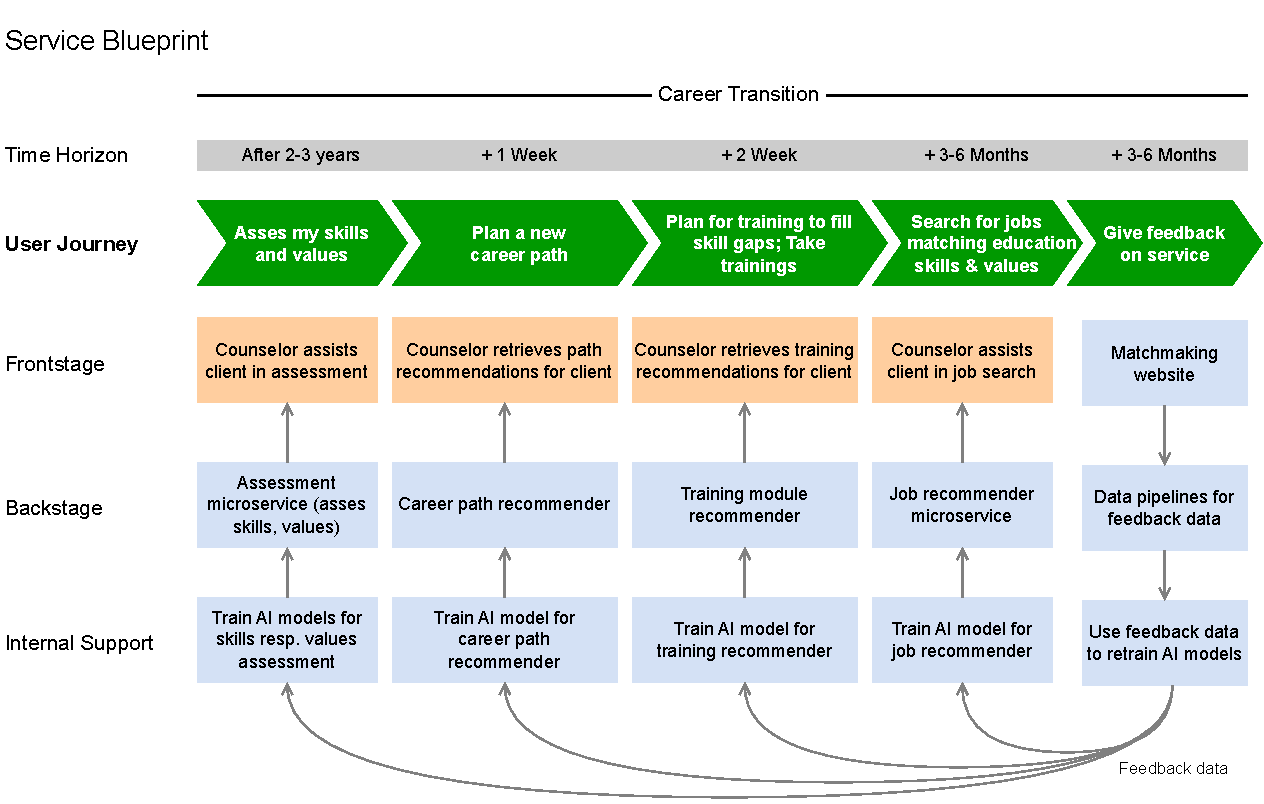
\includegraphics[width=\textwidth]{blueprint_transition.pdf}
    \end{figure}
\end{landscape}


Based on the pricing and estimated usage proportion of each API endpoint, we can estimate the
average price per API request to be 1.075 USD. Further, each market entry customer journey may
bring revenues of 9.00 USD, considering that it may need 20 job recommendations in average. The
writing assistance for CVs and application letters is free to use as it is not embedded in the
CCaaS API but in the LinkedIn job application forms. The career transition customer journey may
bring revenues of 15.50 USD, considering that it may need 5 training recommendations and 20 job
recommendations in average. The market entry customer journey is expected to be used more often
than the career transition customer journey, as the latter is only relevant for a subset of the
market entry customers. The average revenue per customer journey is thus estimated to be 10.95 USD,
considering 70\% market entry customer journeys and 30\% career transition customer journeys.

\subsection{System Architecture}
\label{subsec:system_architecture}

CCaaS is built as a series of microservices that each handle different types of recommendation
tasks using narrow AI models specifically designed and trained for that task. The services are 
built along the lines of the core value proposition of CCaaS identified in Sections \ref{sec:enablers}
\& \ref{sec:business_model}, namely providing career assessments, career path recommendations, training
recommendations, job recommendations, and writing assistance for CVs and application letters. The
microservices' architecture enables containers to be deployed and scaled independently. They are
connected via a message broker that handles the communication between the services and persistent
storage engines (e.g., to store newly created recommendations and log API requests). Two additional
microservices are responsible for the metering of the API usage and the billing and charging of the
API usage fees to the counseling companies. A web application serves as the gatekeeper between
counselors and clients: clients can choose which counselors they want to work with (matchmaking)
as well as grant access to their LinkedIn profile data to the chosen counselor, so that counselors 
can then subsequently access the client's data via the API and retrieve user-specific recommendations.

A separate system entails the data extraction, transformation and loading (ETL) pipelines that load 
and transforms user data and job data, and ingest them into a distributed large data storage layer
(data lake). The data lake is used to provide large volumes of data in the right format that is 
required to train the AI models. Training of the AI models happens on a cluster of GPU servers. As
introduced in the Section \ref{sec:business_model}, the GPU server farm is provided by the parent
company Microsoft via Azure cloud computing services. The trained models are then deployed to the
microservices that are responsible for the actual recommendation tasks. The overall system architecture
is shown in Figure~\ref{fig:system_architecture} using the C4 modelling language for software architecture
\citep{brownC4ModelVisualising2010}.

\begin{landscape}
    \begin{figure}
        \centering
        \caption{CCaaS system architecture in C4 Level 2 notation (own illustration).}
        \label{fig:system_architecture}
        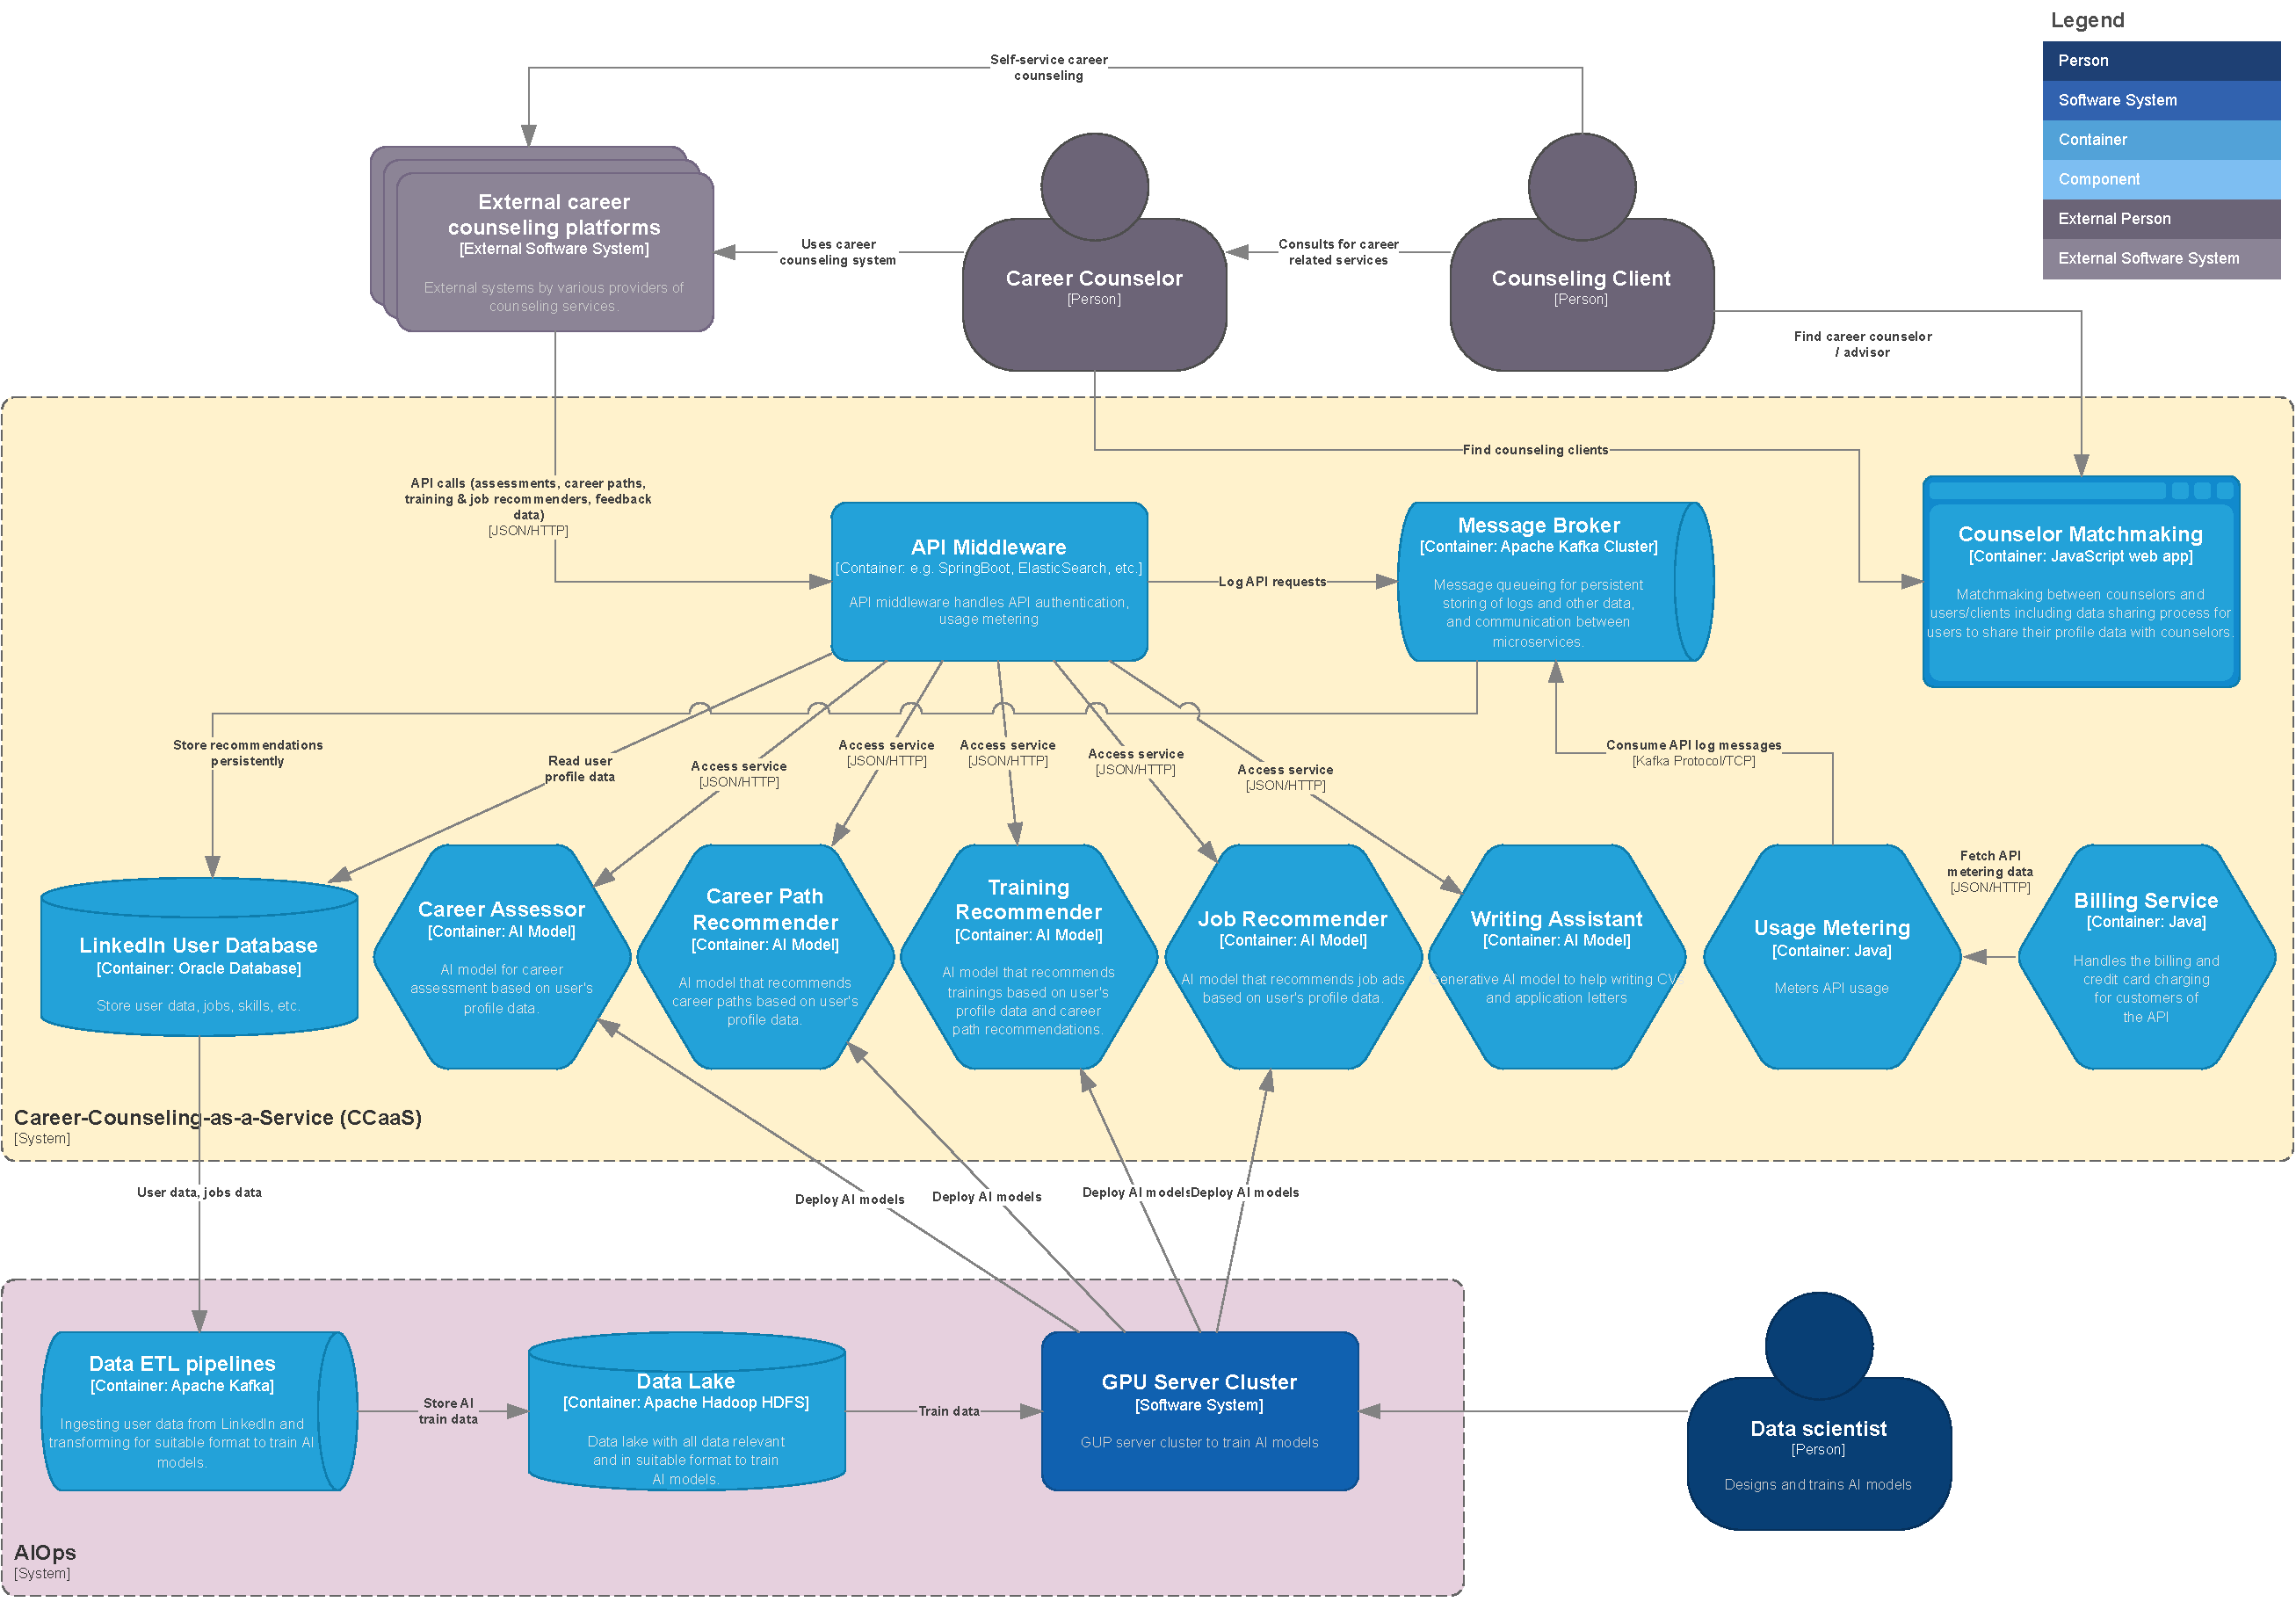
\includegraphics[width=\textwidth]{figures/c4_system_architecture.pdf}
    \end{figure}        
\end{landscape}


